\section{Estimating the critical rate from learned fields}
\label{sec:estimators}

A diffusion model provides a learned score $s_\theta \approx s$, and a second output can be trained to give $m_\theta \approx m$ by regressing $f(X_t)$ on $Y_t$. The question is how to combine them into $R$. Write $s_\theta = s + \delta s$, $m_\theta = m + \delta m$, and let $\eta_s = (\E|\delta s|^2/\E|s|^2)^{1/2}$ and $\eta_m$ be the relative $L^2(p_t)$ errors.

\subsection{Two forms}

The \emph{plain form} inserts the learned fields into Eq.~\eqref{eq:R},
\begin{equation}
R_{\rm plain} = \frac{\E[s_\theta\cdot m_\theta]}{\sigma^2\,\E|s_\theta|^2}.
\label{eq:Rplain}
\end{equation}
The \emph{divergence form} first integrates by parts, $\E[s\cdot m] = -\E[\dv m]$ and $\E|s|^2 = -\E[\dv s]$, and then inserts the learned fields,
\begin{equation}
R_{\rm div} = \frac{\E[\dv m_\theta]}{\sigma^2\,\E[\dv s_\theta]} .
\label{eq:Rdiv}
\end{equation}
Both are evaluated with samples of $Y_t$, which a diffusion model has by construction: data plus noise. The divergences are the traces of the Jacobians of the network outputs with respect to $y$, computed exactly through the network.

\begin{proposition}[errors enter the divergence form linearly]
\label{prop:linear}
Let $\delta s$ and $\delta m$ be differentiable fields with $p\,\delta s$ and $p\,\delta m$ vanishing at infinity. Then
\begin{align}
\E[\dv s_\theta] &= -\E|s|^2 - \E[s\cdot\delta s], \nonumber\\
\E[\dv m_\theta] &= -\E[s\cdot m] - \E[s\cdot\delta m],
\label{eq:linear}
\end{align}
whereas
\begin{align}
\E|s_\theta|^2 &= \E|s|^2 + 2\E[s\cdot\delta s] + \eta_s^2\,\E|s|^2, \nonumber\\
\E[s_\theta\cdot m_\theta] &= \E[s\cdot m] + \E[s\cdot\delta m] + \E[\delta s\cdot m] + \E[\delta s\cdot\delta m].
\label{eq:quadratic}
\end{align}
Consequently:
\begin{enumerate}
\item[(a)] for a scale error $s_\theta = (1+\eta)s$, $m_\theta = m$, both forms give $R/(1+\eta)$;
\item[(b)] for errors orthogonal to the true fields and to each other, $\E[s\cdot\delta s] = \E[s\cdot\delta m] = \E[\delta s\cdot m] = \E[\delta s\cdot\delta m] = 0$, the divergence form is exact, $R_{\rm div} = R$, while $R_{\rm plain} = R/(1+\eta_s^2)$.
\end{enumerate}
\end{proposition}
\begin{proof}
$\E[\dv u] = \int p\,\dv u = -\int \nabla p\cdot u = -\E[s\cdot u]$ for any field $u$ with $p u \to 0$; apply it to $u = s + \delta s$ and $u = m + \delta m$. Equation~\eqref{eq:quadratic} is the expansion of the products. For (a), $R_{\rm div} = \E[s\cdot m]/(\sigma^2(1+\eta)\E|s|^2)$ and $R_{\rm plain} = (1+\eta)\E[s\cdot m]/(\sigma^2(1+\eta)^2\E|s|^2)$. For (b), insert the vanishing terms into Eqs.~\eqref{eq:linear} and~\eqref{eq:quadratic}.
\end{proof}

The identities hold for learned fields because the expectation is taken under the \emph{true} law $p_t$, not under the law the network represents. In the divergence form a learned field appears once, and its error enters only through its projection on the true score. In the plain form the score error enters also through its square, $\eta_s^2\E|s|^2$, which is positive and cannot cancel, through the cross term $\E[\delta s\cdot\delta m]$, and through its projection $\E[\delta s\cdot m]$ on $m$ rather than on $s$. An error that oscillates on the scale $\sigma$ is nearly orthogonal to the smooth true fields, which is the situation of part (b): its linear terms largely cancel and only the extra terms of the plain form survive. Proposition~\ref{prop:linear} does not order the two forms for every error; with errors chosen so that the extra terms of the plain form cancel its linear terms, the plain form can come out closer. How the two forms compare for realistic errors is therefore a numerical question, answered next.

\subsection{Required accuracy}

Before training any network, we fixed the accuracy needed by adding artificial errors to the exact fields (Sec.~\ref{sec:learning} describes the exact fields). Three kinds were used: a smooth random field with correlation length $\sigma$ (twenty realizations; we report the 95th percentile of $|\Delta R|$), a scale error $(1+\eta)s$, and, in two dimensions, the exact score of a slightly wider blur. Figure~\ref{fig:required} shows the error of $R$ relative to the margin. For the scale error the two forms coincide, as Proposition~\ref{prop:linear}(a) states. For smooth random errors, as part (b) suggests, the divergence form is 5 to 16 times more accurate in two dimensions and 11 to 60 times in four dimensions, and in no case we tested is it less accurate. Table~\ref{tab:required} lists the largest $\eta$ that keeps $|\Delta R|$ below $10\%$ and $50\%$ of the margin for every kind of error. It is set by the scale error in four dimensions and therefore is the same for both forms there.

\begin{figure*}[t]
\centering
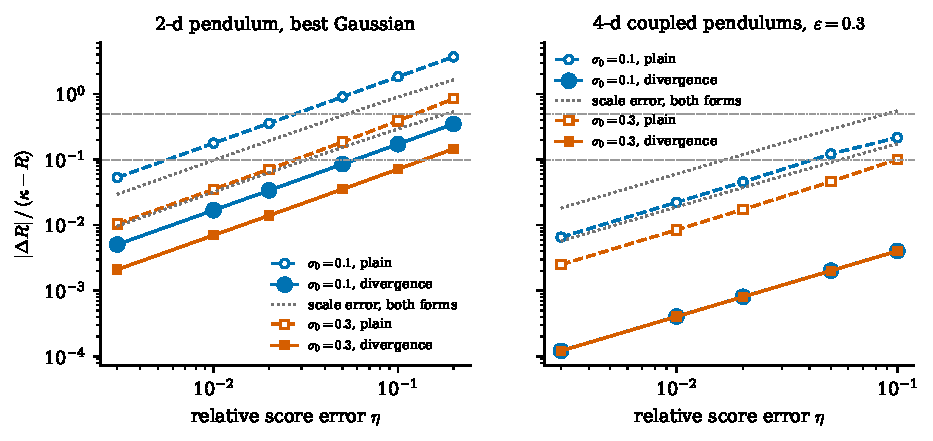
\includegraphics[width=0.85\textwidth]{figures/fig1_required_accuracy.pdf}
\caption{Error of the critical rate, relative to the margin $\kappa - R$, for a smooth random error of relative size $\eta$ in the score (95th percentile over twenty realizations, correlation length $\sigma$). Open symbols, dashed: plain form, Eq.~\eqref{eq:Rplain}. Filled symbols, solid: divergence form, Eq.~\eqref{eq:Rdiv}. Dotted: a scale error $(1+\eta)s$, for which both forms give $R/(1+\eta)$ exactly. Horizontal lines: $10\%$ and $50\%$ of the margin. Left: pendulum, best Gaussian state. Right: coupled pendulums, $\varepsilon = 0.3$, $W = 3$ state (Sec.~\ref{sec:fourdim}).}
\label{fig:required}
\end{figure*}

\begin{table}[t]
\caption{Required accuracy: the largest relative error $\eta$ (from the scanned values $0.003$, $0.01$, $0.02$, $0.05$, $0.1$, $0.2$) for which $|\Delta R|$ stays below $10\%$ / $50\%$ of the margin for every kind of error, at $t = 0$. Divergence form. ``$<$'': even $\eta = 0.003$ exceeds the criterion.}
\label{tab:required}
\begin{ruledtabular}
\begin{tabular}{llcc}
state & $\sigma_0$ & score & $m$ \\
\hline
pend., Gaussian & $0.3$ & $0.02$ / $0.1$ & $0.02$ / $0.1$ \\
 & $0.1$ & $0.01$ / $0.02$ & $0.003$ / $0.02$ \\
 & $0.03$ & $<$ / $0.01$ & $<$ / $0.003$ \\
pend., fan & $0.3$ & $0.02$ / $0.1$ & $0.02$ / $0.1$ \\
 & $0.1$ & $0.003$ / $0.02$ & $0.003$ / $0.02$ \\
coupled, $\varepsilon\!=\!0.1$ & $0.3$ & $0.02$ / $0.1$ & $0.02$ / $0.1$ \\
 & $0.1$ & $0.01$ / $0.05$ & $0.01$ / $0.05$ \\
coupled, $\varepsilon\!=\!0.3$ & $0.3$ & $0.05$ / $0.1$ & $0.05$ / $0.1$ \\
 & $0.1$ & $0.01$ / $0.05$ & $0.01$ / $0.05$ \\
\end{tabular}
\end{ruledtabular}
\end{table}

The table sets the target for learning: relative errors of about $1\%$ at $\sigma_0 = 0.1$ and a few percent at $\sigma_0 = 0.3$. At $\sigma_0 = 0.03$ the target is below $0.3\%$, which our networks did not reach (Sec.~\ref{sec:twodim}).
